\documentclass[aspectratio=43, xcolor=table]{beamer}
%\usepackage[english]{babel}

%Cargar paquetes
\usepackage[utf8]{inputenc}%Permite usar acentos
\usepackage[spanish]{babel}%Configura el idioma por defecto a español
\usepackage{amsmath}%Introduce términos matemáticos
\usepackage{graphicx}%Permite introducir figuras
\usepackage[options]{natbib}%Bibliografía con estilos %No funcionan estilos en Beamer
\newcommand{\grad}{\hspace{-2mm}$\phantom{a}^{\circ}$}

\usepackage{amsthm}
\usepackage{mathtools}
\usepackage{physics}
\usepackage{calligra}
\usepackage{csquotes}
\usepackage{tensor}
\usepackage[thicklines]{cancel}
\usepackage{tcolorbox}
\usepackage{pstricks}
\usepackage[backend=biber, bibstyle=nature, sorting=nty, citestyle=numeric-comp]{biblatex} %Custom bibliography
    \addbibresource{bib.bib} %Load references


\DeclareMathAlphabet{\mathcalligra}{T1}{calligra}{m}{n}
\DeclareFontShape{T1}{calligra}{m}{n}{<->s*[2.2]callig15}{}
\newcommand{\scriptr}{\mathcalligra{r}\,}
\newcommand{\boldscriptr}{\pmb{\mathcalligra{r}}\,}
\def\rc{\scriptr}
\def\brc{\boldscriptr}
\def\hrc{\hat\brc}
\newcommand{\ie}{\emph{i.e.}} %id est
\newcommand{\eg}{\emph{e.g.}} %exempli gratia
\newcommand{\rtd}[1]{\ensuremath{\left\lfloor #1 \right\rfloor}}
\newcommand{\dirac}[1]{\ensuremath{\delta \left( #1 \right)}}
\newcommand{\diract}[1]{\ensuremath{\delta^3 \left( #1 \right)}}
\newcommand{\e}{\ensuremath{\epsilon_0}}
\newcommand{\m}{\ensuremath{\mu_0}}
\newcommand{\V}{\ensuremath{\mathcal{V}}}
\newcommand{\prnt}[1]{\ensuremath{\left(#1\right)}} %parentheses
\newcommand{\colch}[1]{\ensuremath{\left[#1\right]}} %square brackets
\newcommand{\chave}[1]{\ensuremath{\left\{#1\right\}}}  %curly brackets

\useoutertheme{infolines}
\useinnertheme{rectangles}
\usefonttheme{professionalfonts}


\definecolor{orange}{HTML}{f28165}
\definecolor{gray}{HTML}{303030}
\definecolor{yellow}{HTML}{f0be52}
\definecolor{lightorange}{HTML}{f19e58}

\renewcommand{\CancelColor}{\color{orange}}

\makeatletter
\newcommand{\mybox}[1]{%
  \setbox0=\hbox{#1}%
  \setlength{\@tempdima}{\dimexpr\wd0+13pt}%
  \begin{tcolorbox}[colback=orange,colframe=orange,boxrule=0.5pt,arc=4pt,
      left=6pt,right=6pt,top=6pt,bottom=6pt,boxsep=0pt,width=\@tempdima]
    \textcolor{white}{#1}
  \end{tcolorbox}
}
\makeatother

\usecolortheme[named=orange]{structure}
\usecolortheme{sidebartab}
\usecolortheme{orchid}
\usecolortheme{whale}
\setbeamercolor{alerted text}{fg=yellow}
\setbeamercolor{block title alerted}{bg=alerted text.fg!90!black}
\setbeamercolor{block title example}{bg=lightorange!60!black}
\setbeamercolor{background canvas}{bg=gray}
\setbeamercolor{normal text}{bg=gray,fg=white}

\setbeamertemplate{footline}
        {
      \leavevmode%
      \hbox{%
      \begin{beamercolorbox}[wd=.333333\paperwidth,ht=2.25ex,dp=1ex,center]{author in head/foot}%
        \usebeamerfont{author in head/foot}\insertshortauthor~~(\insertshortinstitute)
      \end{beamercolorbox}%
      \begin{beamercolorbox}[wd=.333333\paperwidth,ht=2.25ex,dp=1ex,center]{title in head/foot}%
        \usebeamerfont{title in head/foot}\insertshorttitle
      \end{beamercolorbox}%
      \begin{beamercolorbox}[wd=.333333\paperwidth,ht=2.25ex,dp=1ex,center]{date in head/foot}%
        \usebeamerfont{page number in head/foot}\insertframenumber/\inserttotalframenumber%\hspace*{2em}

    %#turning the next line into a comment, erases the frame numbers
        %\insertframenumber{} / \inserttotalframenumber\hspace*{2ex} 

      \end{beamercolorbox}}%
      \vskip0pt%
    }


\setbeamertemplate{blocks}[rectangle]
\setbeamercovered{dynamic}

\setbeamertemplate{section page}
{
	\begin{centering}
		\begin{beamercolorbox}[sep=27pt,center]{part title}
			\usebeamerfont{section title}\insertsection\par
			\usebeamerfont{subsection title}\insertsubsection\par
		\end{beamercolorbox}
	\end{centering}
}

%\setbeamertemplate{subsection page}
%{
%	\begin{centering}
%		\begin{beamercolorbox}[sep=12pt,center]{part title}
%			\usebeamerfont{subsection title}\insertsubsection\par
%		\end{beamercolorbox}
%	\end{centering}
%}

\newcommand{\hlight}[1]{\colorbox{violet!50}{#1}}
\newcommand{\hlighta}[1]{\colorbox{red!50}{#1}}
\title{Modelado conceptual con BPMN} %->->->->-> Check hyperref title <-<-<-<-<-
%\subtitle{And Some Things About It}
\author[C.J. Uribe-Martes]{Carlos Javier Uribe Martes}
\institute[CUC]{
    Ingeniería Industrial%
    \\%
    Universidad de la Costa%
} %You can change the Institution if you are from somewhere else
\date{Marzo 01, 2020}
%\logo{\includegraphics[width= 0.2\textwidth]{images/a-logo.png}}

\begin{document}
    
    \frame{\titlepage}
    
    \begin{frame}{Contenido}
        \tableofcontents
    \end{frame}
    
    \section{Modelado conceptual}

\begin{frame}{Introducción}
    \begin{itemize}
        \item Se tiene información y tiempo limitado para pretender modelar el sistema completo.
	    \item Incluso ante suficiente tiempo e información, a menudo un modelo más sencillo (respecto a la complejidad del sistema real) basta para el problema en estudio.
	    \item Al desarrollar un modelo más simple se debe definir el nivel de abstracción al que funcionará.
    \end{itemize}
\end{frame}

\begin{frame}{Definición}
    \begin{itemize}
        \item Un modelo conceptual es una \textit{descripción del modelo de simulación, no específica de un software, que describe los objetivos, entradas, salidas, contenido, supuestos y simplificaciones del modelo}.
        \item Es la abstracción de la parte del sistema que va a representar el modelo de simulación e implica una representación simplificada del sistema real.
    	%\item Es la actividad de decidir qué modelar y qué no modelar.
    \end{itemize}
\end{frame}

\begin{frame}{Requerimientos}
    \begin{itemize}
        \item Un buen modelo conceptual debe:
        \begin{itemize}
        \item Producir resultados precisos para el objetivo propuesto (validez).
        \item Ser creido por los clientes (credibilidad).
        \item Ser factible de construir dentro de las limitaciones de información y de tiempo (factibilidad).
        \item Tener utilidad, es decir, ser fácil de usar, flexible, visual y rápido de ejecutar (usabilidad).
        \end{itemize}
    \end{itemize}
\end{frame}

\begin{frame}{Documentación del modelo conceptual}
    \begin{itemize}
        \item El modelo conceptual no siempre se expresa explícitamente.
	    %\item Es una buena práctica documentar el modelo conceptual y, al hacerlo, proporcionar un medio de comunicación entre todas las partes en un estudio de simulación. 
	    \item Provee un medio de comunicación entre todas las partes involucradas en el estudio de simulación.
    \end{itemize}
    \begin{figure}
        \centering
        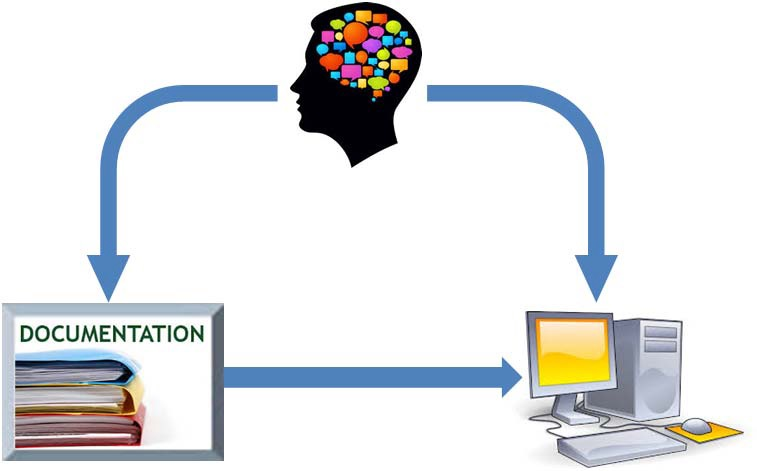
\includegraphics[width=6cm]{images/whereisthemodel.jpg}
        \caption{¿Dónde está el modelo? Tomado de \cite{robinson}}
        %\label{fig:my_label}
    \end{figure}
\end{frame}

\begin{frame}{Documentación del modelo conceptual}
    \begin{itemize}
	    \item No hay estándares establecidos para documentar modelos conceptuales, pero se han propuesto una variedad de enfoques, que incluyen:
	    \begin{enumerate}
	        \item Lista de componentes.
	        \item Diagrama de flujo de procesos.
	        \item Diagrama de actividades.
	        \item Lenguaje unificado de modelado (UML).
	        \item Redes de Petri.
	    \end{enumerate}
    \end{itemize}
\end{frame}
    
    \section{BPMN}

\begin{frame}{BPMN}
    \begin{itemize}
        \item Son las siglas para Business Process Modeling Notation.
	    \item Es un lenguaje para facilitar la comunicación de los procesos en forma clara, completa y eficiente.
	\end{itemize}
\end{frame}

\begin{frame}{Elementos de un diagrama BPMN}
    \begin{itemize}
        \item Un diagrama BPMN está compuesto por tres elementos básicos, que son los objetos de flujo (eventos, actividades y compuertas), además de objetos conectores y reglas de construcción. 
    \end{itemize}
\end{frame}

\subsection{Eventos}

\begin{frame}{Eventos}
    \begin{itemize}
        \item Representan algo que ocurre o puede ocurrir durante el curso del proceso.
        \item Suelen tener una causa o un resultado.
        \item De acuerdo con el momento en que afectan al flujo, se dividen en tres tipos:
        \begin{enumerate}
            \item Eventos de inicio.
            \item Eventos intermedios.
            \item Eventos de fin.
        \end{enumerate}
    \end{itemize}
\end{frame}

\begin{frame}{Eventos de inicio}
    \begin{itemize}
        \item Representa el disparador de un proceso. Todo proceso debe tener al menos un evento de inicio.
    \end{itemize}
    \begin{figure}
        \centering
        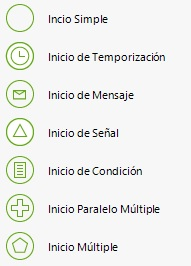
\includegraphics[scale=0.8]{images/event_start.jpg}
        %\caption{Caption}
        %\label{fig:my_label}
    \end{figure}
\end{frame}

\begin{frame}{Eventos intermedios}
    \begin{itemize}
        \item Ocurren a la mitad del proceso, forman parte directa del flujo del proceso.
    \end{itemize}
    \begin{figure}
        \centering
        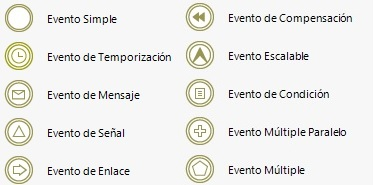
\includegraphics[scale=0.8]{images/event_intermediate.jpg}
        %\caption{Caption}
        %\label{fig:my_label}
    \end{figure}    
\end{frame}

\begin{frame}{Eventos de fin}
    \begin{itemize}
        \item Identifican el fin del proceso. 
        \item Todo proceso debe tener al menos un evento de fin, pero es común que tengan varios para dar claridad al tipo de terminación que tuvo el proceso.
    \end{itemize}
    \begin{figure}
        \centering
        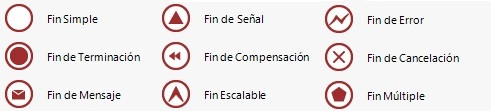
\includegraphics[scale=0.8]{images/event_final.jpg}
        %\caption{Caption}
        %\label{fig:my_label}
    \end{figure}
\end{frame}

\subsection{Actividades}

\begin{frame}{Actividades}
    \begin{itemize}
        \item Es un término genérico para el trabajo que se realiza en el proceso. 
        \item Representado por un rectángulo redondeado. 
        \item Puede ser:
            \begin{itemize}
                \item Tareas.
                \item Subprocesos.
            \end{itemize}
    \end{itemize}
    
\end{frame}

\begin{frame}{Tareas}
    \begin{itemize}
        \item Representan el trabajo que consume recursos de la organización.
        \item Cuando una actividad es completada la siguiente actividad inicia.
    \end{itemize}
    \begin{figure}
        \centering
        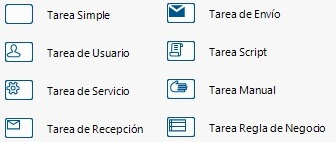
\includegraphics[scale=0.8]{images/task.jpg}
        %\caption{Caption}
        %\label{fig:my_label}
    \end{figure}
\end{frame}

\begin{frame}{Subprocesos}
    \begin{itemize}
        \item Es una actividad compuesta incluida dentro de un proceso.
        \item Incluye a su vez un conjunto de actividades y una secuencia lógica, por lo que dicha actividad puede ser analizada a nivel más fino.
    \end{itemize}
    \begin{figure}
        \centering
        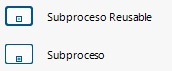
\includegraphics[scale=0.8]{images/subprocess.jpg}
        %\caption{Caption}
        %\label{fig:my_label}
    \end{figure}
\end{frame}

\subsection{Compuertas}

\begin{frame}{Compuertas}
    \begin{itemize}
        \item Controlan los puntos de divergencia y de convergencia del flujo.
    \end{itemize}
    \begin{figure}
        \centering
        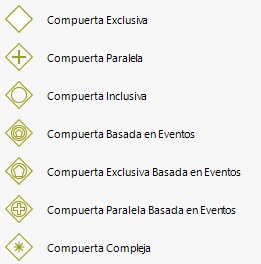
\includegraphics[scale=0.8]{images/gateway.jpg}
        %\caption{Caption}
        %\label{fig:my_label}
    \end{figure}
\end{frame}

\subsection{Objetos conectores}

\begin{frame}{Objetos conectores}
    \begin{itemize}
        \item Conectan los objetos de flujo de un proceso, y definen el orden de ejecución de las actividades. Pueden ser:
        \begin{itemize}
            \item Secuencia: Muestra el orden de los eventos, actividades, decisiones que se realizan dentro del proceso.
            \item Mensaje: Identifica el flujo de mensajes entre las distintas partes de los procesos.
            \item Asociación: Asocia artefactos con objetos de flujo.
        \end{itemize}
    \end{itemize}
    \begin{figure}
        \centering
        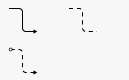
\includegraphics[scale=0.8]{images/flows.jpg}
        %\caption{Caption}
        %\label{fig:my_label}
    \end{figure}
\end{frame}

\subsection{Reglas}

\begin{frame}{Reglas}
    \begin{itemize}
        \item Un \textit{pool} contiene un único proceso y su nombre puede considerarse como el nombre del proceso.
        \item Los canales (\textit{lanes}) representan a cada uno de los participantes del proceso. Puede representar un área funcional, un cargo o un rol.
        \item Las fases se utilizan para delimitar las etapas distintas de un proceso, en donde se puede identificar una salida intermedia entre una etapa y la siguiente.
    \end{itemize}
    \begin{figure}
        \centering
        
\includegraphics[scale=0.8]{images/rules.jpg}
        %\caption{Caption}
        %\label{fig:my_label}
    \end{figure}
\end{frame}
    
    %\section{Modelos de inventario}

\begin{frame}{Simulación de un modelo de inventarios}
    \begin{itemize}
        \item Los estados del sistema se refieren al nivel de inventario actual, pedidos pendientes, existencia de \textit{backorders}.
        \item Los eventos que pueden ocurrir se relacionan con la demanda de unidades del inventario, la revisión de la posición del inventario y la decisión resultante de hacer una orden y la llegada de un pedido.
    \end{itemize}
\end{frame}

\begin{frame}{Sistema de inventarios $(s,S)$}
    \begin{itemize}
        \item Una política de inventarios $(s,S)$, es un sistema de revisión continua.
        \item Si el inventario se encuentra en un nivel igual o menor que $s$ se solicitan suficientes unidades para llevar el inventario a un nivel $S$.
        \item El \textit{lead time}, $l$, puede ser variable.
        \item La demanda por lo general no se conoce con certeza, por lo que puede modelarse a través de una variable aleatoria.
        \item Puede o no admitirse la ocurrencia de \textit{backorders}.
    \end{itemize}
\end{frame}

\begin{frame}{Sistema de inventarios $(s,S)$}
    \begin{figure}
        \centering
        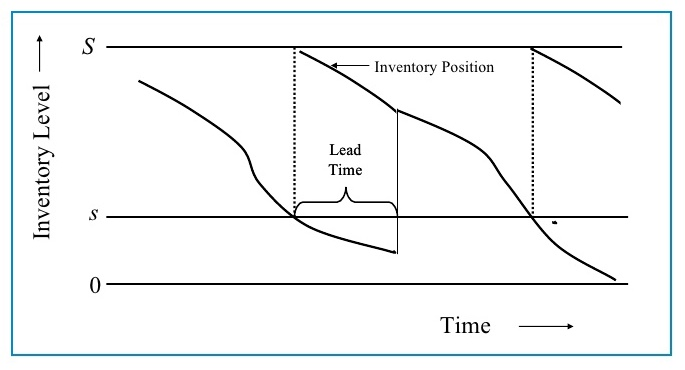
\includegraphics[width=10cm]{images/inventory-management12248440536560389-73-728-2.jpg}
        %\caption{Caption}
        \label{fig:my_label}
    \end{figure}
\end{frame}

\begin{frame}{Parámetros de interés}
    \begin{itemize}
        \item Las políticas de inventario tienen varios parámetros, algunos controlables y otros no.
        \item Entre los parámetros controlables se encuentran:
        \begin{itemize}
            \item Inventario máximo, $S$.
            \item Inventario de seguridad, $s$.
            \item Lead time, $l$.
            \item Periodo de revisión, $t$.
        \end{itemize}
    \end{itemize}
\end{frame}

\begin{frame}{Tabla de simulación para un modelo de inventarios}{}

{\footnotesize
\begin{table}[]
\begin{tabular}{|l|c|c|c|c|c|c|}
\hline
\rowcolor[HTML]{794033} 
{\color[HTML]{FFFFFF} \begin{tabular}[c]{@{}l@{}}Día\\ (rlj)\end{tabular}} &  \multicolumn{1}{l|}{\cellcolor[HTML]{794033}{\color[HTML]{FFFFFF} \begin{tabular}[c]{@{}l@{}}Inv. \\ inicial\\ (estado)\end{tabular}}} & \multicolumn{1}{l|}{\cellcolor[HTML]{794033}{\color[HTML]{FFFFFF} \begin{tabular}[c]{@{}l@{}}Demanda\\ (entrada)\end{tabular}}} & \multicolumn{1}{l|}{\cellcolor[HTML]{794033}{\color[HTML]{FFFFFF} \begin{tabular}[c]{@{}l@{}}Inv. \\ final\\ (est.)\end{tabular}}} & \multicolumn{1}{l|}{\cellcolor[HTML]{794033}{\color[HTML]{FFFFFF} \begin{tabular}[c]{@{}l@{}}Faltante\\ (estado)\end{tabular}}} & \multicolumn{1}{l|}{\cellcolor[HTML]{794033}{\color[HTML]{FFFFFF} \begin{tabular}[c]{@{}l@{}}Orden \\ pend.\\ (est.)\end{tabular}}} & \multicolumn{1}{l|}{\cellcolor[HTML]{794033}{\color[HTML]{FFFFFF} \begin{tabular}[c]{@{}l@{}}Días para \\ llegada \\ orden\\ (estado)\end{tabular}}} \\ \hline
\rowcolor[HTML]{F28165} 
{\color[HTML]{FFFFFF} 0} & {\color[HTML]{FFFFFF} -} & {\color[HTML]{FFFFFF} -} & {\color[HTML]{FFFFFF} 3} & {\color[HTML]{FFFFFF} 0} & {\color[HTML]{FFFFFF} 8} & {\color[HTML]{FFFFFF} 2} \\ \hline
\rowcolor[HTML]{F28165} 
{\color[HTML]{FFFFFF} 1} & {\color[HTML]{FFFFFF} 3} & {\color[HTML]{FFFFFF} 2} & {\color[HTML]{FFFFFF} 1} & {\color[HTML]{FFFFFF} 0} & {\color[HTML]{FFFFFF} 8} & {\color[HTML]{FFFFFF} 1} \\ \hline
\rowcolor[HTML]{F28165} 
{\color[HTML]{FFFFFF} 2} & {\color[HTML]{FFFFFF} 1} & {\color[HTML]{FFFFFF} 1} & {\color[HTML]{FFFFFF} 8} & {\color[HTML]{FFFFFF} 0} & {\color[HTML]{FFFFFF} } & {\color[HTML]{FFFFFF} } \\ \hline
\rowcolor[HTML]{F28165} 
{\color[HTML]{FFFFFF} 3} & {\color[HTML]{FFFFFF} 8} & {\color[HTML]{FFFFFF} 2} & {\color[HTML]{FFFFFF} 6} & {\color[HTML]{FFFFFF} 0} & {\color[HTML]{FFFFFF} } & {\color[HTML]{FFFFFF} } \\ \hline
\rowcolor[HTML]{F28165} 
{\color[HTML]{FFFFFF} 4} & {\color[HTML]{FFFFFF} 6} & {\color[HTML]{FFFFFF} 1} & {\color[HTML]{FFFFFF} 5} & {\color[HTML]{FFFFFF} 0} & {\color[HTML]{FFFFFF} } & {\color[HTML]{FFFFFF} } \\ \hline
\rowcolor[HTML]{F28165} 
{\color[HTML]{FFFFFF} 5} & {\color[HTML]{FFFFFF} 5} & {\color[HTML]{FFFFFF} 2} & {\color[HTML]{FFFFFF} 3} & {\color[HTML]{FFFFFF} 0} & {\color[HTML]{FFFFFF} 8} & {\color[HTML]{FFFFFF} 1} \\ \hline
\rowcolor[HTML]{F28165} 
{\color[HTML]{FFFFFF} 6} & {\color[HTML]{FFFFFF} 3} & {\color[HTML]{FFFFFF} 3} & {\color[HTML]{FFFFFF} 8} & {\color[HTML]{FFFFFF} 0} & {\color[HTML]{FFFFFF} } & {\color[HTML]{FFFFFF} } \\ \hline
\rowcolor[HTML]{F28165} 
{\color[HTML]{FFFFFF} 7} & {\color[HTML]{FFFFFF} 8} & {\color[HTML]{FFFFFF} 2} & {\color[HTML]{FFFFFF} 6} & {\color[HTML]{FFFFFF} 0} & {\color[HTML]{FFFFFF} } & {\color[HTML]{FFFFFF} } \\ \hline
\rowcolor[HTML]{F28165} 
{\color[HTML]{FFFFFF} 8} & {\color[HTML]{FFFFFF} 6} & {\color[HTML]{FFFFFF} 3} & {\color[HTML]{FFFFFF} 3} & {\color[HTML]{FFFFFF} 0} & {\color[HTML]{FFFFFF} 8} & {\color[HTML]{FFFFFF} 2} \\ \hline
\rowcolor[HTML]{F28165} 
{\color[HTML]{FFFFFF} 9} & {\color[HTML]{FFFFFF} 3} & {\color[HTML]{FFFFFF} 2} & {\color[HTML]{FFFFFF} 1} & {\color[HTML]{FFFFFF} 0} & {\color[HTML]{FFFFFF} 8} & {\color[HTML]{FFFFFF} 1} \\ \hline
\rowcolor[HTML]{F28165} 
{\color[HTML]{FFFFFF} 10} & {\color[HTML]{FFFFFF} 1} & {\color[HTML]{FFFFFF} 3} & {\color[HTML]{FFFFFF} 6} & {\color[HTML]{FFFFFF} 0} & {\color[HTML]{FFFFFF} } & {\color[HTML]{FFFFFF} } \\ \hline
\end{tabular}
\end{table}}
\end{frame}


\begin{frame}{Medidas de desempeño}
    \begin{itemize}
        \item Algunas medidas de desempeño de interés son:
        \begin{itemize}
            \item Ingresos totales por ventas.
            \item Costos totales de la política de inventario.
            \item Inventario a la mano promedio.
            \item Nivel de backorders promedio.
            \item Ciclo del inventario promedio.
        \end{itemize}
    \end{itemize}
\end{frame}

    
    \section*{Referencias} %You can remove this if you do not want to use it
    \nocite{freund}
        \begin{frame}{Referencias}
            \printbibliography
        \end{frame}
     
    \section{}   
        \begin{frame}{}
            \begin{figure}
                \centering
                
\includegraphics[width=6cm]{images/model.png}
                %\caption{Caption}
                %\label{fig:my_label}
            \end{figure}
        \end{frame}

\end{document}
